
\section{Iniciar Sesión}
El inicio de sesión del usuario permite al actor ingresar a la aplicación y de esta manera podrá desempeñar las acciones correspondientes a su rol.

\subsubsection{Procedimiento}
\begin{enumerate}
	
	\item Ingresa el correo electrónico y la contraseña previamente registrados en la pantalla \textbf{Iniciar Sesión}.
	
	\begin{figure}[!htbp]			\hypertarget{fig:IniciarSesion2}{\hspace{1pt}}
		\begin{center}
			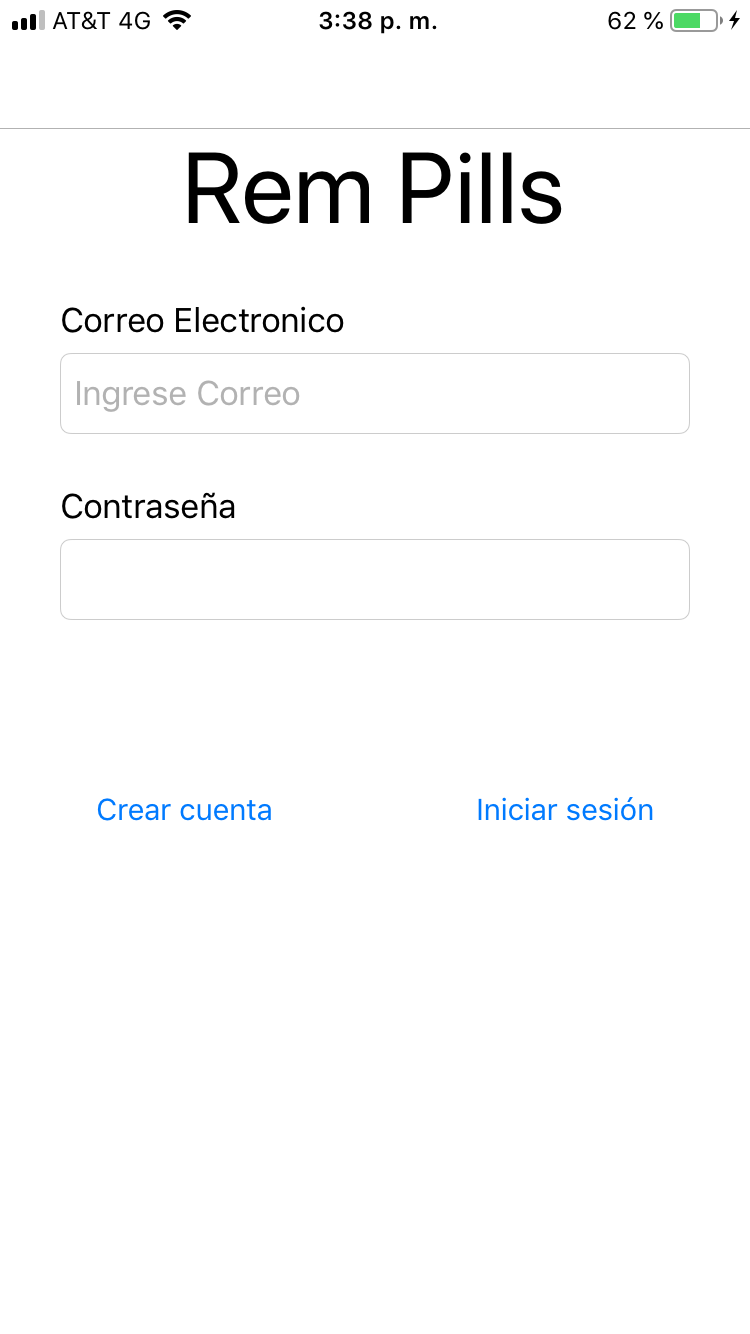
\includegraphics[height=0.4\textheight]{Paciente/IniciarSesion/images/IMG-3180}
			\caption{Iniciar Sesión}
			\label{fig:IniciarSesion2}
		\end{center}
	\end{figure}

	\item Presiona el botón \textbf{Iniciar Sesión}.
	
	\item Se mostrará la pantalla \textbf{Menú Principal del Doctor}.
	\newpage
		\begin{figure}[!htbp]			\hypertarget{fig:mpDoctor}{\hspace{1pt}}
		\begin{center}
			\includegraphics[height=0.4\textheight]{images/Iconos/Advertencia}
			\caption{Menú Principal Doctor}
			\label{fig:mpDoctor}
		\end{center}
	\end{figure}


\end{enumerate}

